\documentclass{beamer}

\usetheme{CambridgeUS}
\usefonttheme{professionalfonts}

\usepackage{graphicx}
\usepackage[miktex]{gnuplottex}
\ShellEscapetrue
\usepackage{epstopdf}
\usepackage{minted}

\usemintedstyle{manni}
\definecolor{mintedBg}{rgb}{0.98,0.98,0.70}

\begin{document}
\title{Automatic Differentiation beyond typedef and operator overloading}
\author{Peter Caspers}
\institute{Quaternion}
\date{November 30, 2015}

\frame{\titlepage}

\frame{\frametitle{Table of contents}\tableofcontents[hideallsubsections]}

\section{Introduction to AD}

\begin{frame}[fragile]
\frametitle{AD in a nutshell}
\begin{itemize}
\item compute derivatives by symbolic differentiation of the operation sequence ($+*-/$, $\exp, \sin, ...$) using the chain rule
\item derivatives can be propagated in forward and reverse (adjoint) mode
\item results are exact up to machine precision, also for higher order derivatives
\item law of cheap gradient in adjoint mode (complexity = constant low multiple\footnote{theory says that the multiple is bounded by 4} of one function evaluation)
\end{itemize}
\end{frame}

\section{Approaches in QuantLib}

\begin{frame}[fragile]
\frametitle{The typedef approach}
\begin{itemize}
\item just says \verb+typedef CppAD::AD<double> Real+
\item it is a bit more complicated than that
\item QuantLibAdjoint project (CompatibL)
\item \textit{AD-or-not-AD} decision at compile time and globally, i.e. no selective activation of variables
\end{itemize}
\end{frame}

\begin{frame}[fragile]
\frametitle{Matrix multiplication with (sleeping) active doubles}
\begin{minted}[bgcolor=mintedBg,fontsize=\footnotesize]{c++}
    Matrix_t<T> A(1024, 1024);
    Matrix_t<T> B(1024, 1024);
    ...
    Matrix_t<T> C = A * B;
\end{minted}
\begin{itemize}
\item \verb+T = double+: 764 ms
\item \verb+T = CppAD::AD<double>:+ 8960 ms
\item Penalty: 11.7x
\item the compiler does not seem to apply certain optimizations to the active type that are possible for the native double (SIMD instructions)
\item this is not an exception, but seems to occur for every ``numerically intense'' code section (see below for a second example)
\end{itemize}
\end{frame}

\begin{frame}[fragile]
\frametitle{The template approach}
\begin{itemize}
\item introduce templated versions of relevant classes (e.g. \verb+Matrix_t+)
\item for backward compatibility, \verb+typedef Matrix_t<Real> Matrix+
\item it is a bit more complicated than that
\item allows mixing of active and native classes, as required, i.e. activation of variables in selected parts of the application only
\item currently not finalized, but basic IRD stuff works (like yield and volatility termstructures, swaps, CMS coupons, GSR model)
\item \url{https://github.com/pcaspers/quantlib/tree/adjoint}
\end{itemize}
\end{frame}

\begin{frame}[fragile]
\frametitle{Expensive gradients with operator overloading}
\begin{itemize}
\item both approaches use operator overloading tools (like CppAD)
\item for numerically intense algorithms, we observe dramatic performance loss (because less optimization can be applied to non-native types)
\item e.g. a convolution engine for bermudan swaptions is 80x slower\footnote{see \tiny\url{https://quantlib.wordpress.com/2015/04/14/adjoint-greeks-iv-exotics}}
in adjoint mode compared to one native-double pricing
\item if AD is actually not needed, the template approach is the way out, otherwise we need other techniques
\end{itemize}
\end{frame}

\section{Source code transformation}

\begin{frame}[fragile]
\frametitle{Source Code Transformation}
\begin{itemize}
\item generate adjoint code at compile time, which hopefully yields better performance
\item however, does not work out of the box like OO tools
\item no mature tool for C++ (ADIC 2.0 under development)
\item needs specific preparation of code before it can be applied
\end{itemize}
\end{frame}

\begin{frame}[fragile]
\frametitle{OpenAD/F}
\begin{itemize}
\item OpenAD is a language independent AD backend working with abstract xml representations (XAIF) of the computational model
\item OpenAD/F adds a Fortran 90 front end
\item Open Source, proven on large scale real-world models
\item \url{http://www.mcs.anl.gov/OpenAD}
\end{itemize}
\end{frame}

\begin{frame}[fragile]
\frametitle{Steps to use SCT}
\begin{itemize}
\item Isolate the core computational code and reimplement it in Fortran
\item Use OpenAD/F to generate adjoint code, build a separate support library from that
\item Use a wrapper class on the QuantLib side to communicate with the support libary
\end{itemize}
\end{frame}

\begin{frame}[fragile]
\frametitle{LGM Bermudan swaption convolution engine}
\begin{itemize}
\item core computation can be implemented in around 200 lines
\item native interface only using doubles and arrays of doubles
\item input: relevant times $\{t_i\}$, model $\{(H(t_i), \zeta(t_i), P(0,t_i)\}$,
Termsheet, codified as index lists $\{k_i, l_i, ...\}$
\item output: npv, gradient w.r.t. $\{(H(t_i), \zeta(t_i), P(0,t_i)\}$
\end{itemize}
\begin{minted}[bgcolor=mintedBg,fontsize=\footnotesize]{fortran}
subroutine lgm_swaption_engine(n_times, times, modpar, n_expiries, &
     expiries, callput, n_floats, &
     float_startidxes, float_mults, index_acctimes, float_spreads, &
     float_t1s, float_t2s, float_tps, &
     fix_startidxes, n_fixs, fix_cpn, fix_tps, &
     integration_points, stddevs, res)
\end{minted}
\end{frame}

\begin{frame}[fragile]
\frametitle{Building the AD support library}
\resizebox{\textwidth}{!}{
\begin{minipage}{3.5\textwidth}
\begin{figure}
    \centering
        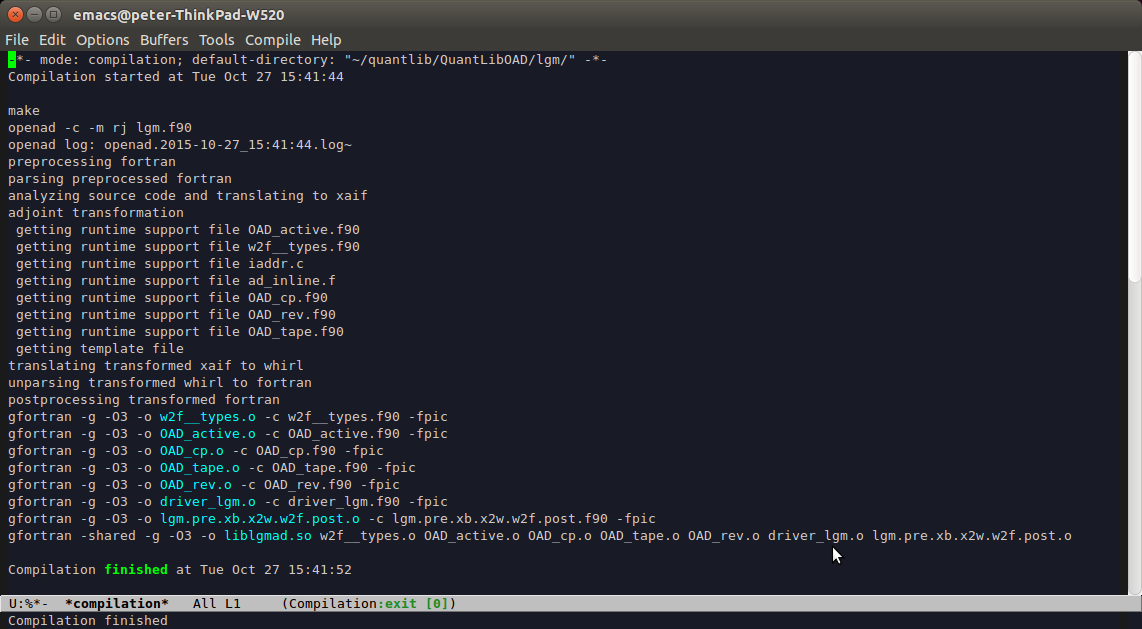
\includegraphics{oad_build.png}
\end{figure}
\end{minipage}}
\end{frame}

\begin{frame}[fragile]
\frametitle{LGM Bermudan swaption convolution engine}
\begin{itemize}
\item C++ wrapper is a normal QuantLib pricing engine
\item precomputes the values for the Fortran interface
\item invokes the Fotran routine
\item stores the npv and the adjoint gradient as results
\end{itemize}
\begin{minted}[bgcolor=mintedBg,fontsize=\tiny]{c++}

void LgmSwaptionEngineAD::calculate() const {
    // collect data needed for core computation routine
    ...
    // join all dates and fill index vectors
    ...
    // call core computation routine and set results

    lgm_swaption_engine_ad_(&ntimes, &allTimes[0], &modpar[0], &nexpiries, ...
                    &integration_pts, &std_devs, &res, &dres[0]);
    ...
    results_.value = res;
    results_.additionalResults["sensitivityTimes"] = allTimes;
    results_.additionalResults["sensitivityH"] = H_sensitivity;
    results_.additionalResults["sensitivityZeta"] = zeta_sensitivity;
    results_.additionalResults["sensitivityDiscount"] = discount_sensitivity;
\end{minted}
\end{frame}

\begin{frame}[fragile]
\frametitle{Performance}
\begin{itemize}
\item 10y bermudan swaption, yearly callable
\item 49 grid points per expiry
\item single pricing\footnote{Intel(R) Core(TM) i7-2760QM CPU @ 2.40GHz, single threaded} (non-transformed code): 4.2 ms
\item pricing + gradient $\in \mathbb{R}^{105}$: 25.6 ms
\item additional stuff\footnote{transformation of gradient w.r.t. model parameters to usual vegas, see below}: 6.2 ms
\item adjoint calculation multiple: 6.1x (7.6x including add. stuff)
\item common, practical target for the adjoint multiple: 5x - 10x
\end{itemize}
\end{frame}

\begin{frame}[fragile]
\frametitle{Where to use AD and where not}
\begin{itemize}
\item apply AD only to differentiable programs
\item avoid to push it through solvers, optimizers, etc.
\item instead use the implicit function theorem to convert gradients w.r.t. calibrated variables to gradients w.r.t. market variables
\item this is more efficient, less error prone (e.g. \verb+Bisection+ produces zero derivatives always, optimizations may produce bogus derivatives depending on the start value)
\item in the case of SCT even necessary from a practical viewpoint
\end{itemize}
\end{frame}

\begin{frame}[fragile]
\frametitle{Calibration of LGM model}
Calibration to $n$ swaptions\footnote{recall that $\zeta(t)$ is the accumulated model variance up to time $t$}
\begin{eqnarray*}
\text{Black}(\sigma_1) - \text{Npv(LGM)}(\zeta_1) &=& 0 \\
... \\
\text{Black}(\sigma_n) - \text{Npv(LGM)}(\zeta_n) &=& 0
\end{eqnarray*}
with
\begin{equation}
\frac{\partial \text{Npv(LGM)}}{\partial \zeta} = \text{diag}(\nu_1, ..., \nu_n), \text{ all } \nu_i \neq 0
\end{equation}
\end{frame}

\begin{frame}[fragile]
\frametitle{Implicit function theorem}
Locally, there exists a unique $g$
\begin{equation}
g(\sigma_1, ... , \sigma_n) = (\zeta_1, ..., \zeta_n)
\end{equation}
and
\begin{equation}
\frac{\partial g}{\partial \sigma} = \left( \frac{\partial \text{Npv(LGM)}}{\partial \zeta} \right) ^ {-1} \frac{\partial \text{Black}}{\partial \sigma}
\end{equation}
\end{frame}

\begin{frame}[fragile]
\frametitle{Pasting the vega together}
\begin{equation*}
\frac{\partial \text{Npv}_\text{Berm}}{\partial \sigma} = \frac{\partial \text{Npv}_\text{Berm}}{\partial \zeta} \frac{\partial \zeta}{\partial \sigma} = \frac{\partial \text{Npv}_\text{Berm}}{\partial \zeta} \left( \frac{\partial \text{Npv}_\text{Calib}}{\partial \zeta} \right) ^ {-1} \frac{\partial \text{Black}}{\partial \sigma}
\end{equation*}
\begin{itemize}
\item the components can be calculated analytically (calibrating swaptions' market vegas) or using the ad engine (calibrating swaptions' $\zeta$-gradient)
\item matrix inversion and multiplication is cheap
\item the additional computation time is quite small (see the example above)
\end{itemize}
\end{frame}

\begin{frame}[fragile]
\frametitle{Summary}
\begin{itemize}
\item global instrumentation (via typedefs) with active variables can lead to performance issues
\item selective / mixed instrumentation (via templates) solves the issue, but leaves problems when AD is required for numerically intense parts of the code
\item source code transformation can solve this issue, an example in terms of a bermudan swaption engine was given using OpenAD/F
\end{itemize}
\end{frame}

\section{Questions}

\begin{frame}[fragile]
\frametitle{Questions / Discussion}
\centerline{thank you for your attention}
\end{frame}
\end{document}
